\documentclass[conference]{IEEEtran}
\usepackage{cite}
\usepackage{amsmath,amssymb}
\usepackage{graphicx}
\usepackage{booktabs}
\usepackage{xcolor}
\usepackage{tikz}
\usetikzlibrary{arrows.meta,positioning}
\usepackage{algorithm}
\usepackage{algpseudocode}
\usepackage{url}
\newcommand{\fillin}[1]{\textcolor{red}{[#1]}}
\newcommand{\safefig}[2]{\IfFileExists{#1}{\includegraphics[width=#2]{#1}}{\fbox{\parbox{#2}{\centering\footnotesize figure missing}}}}
\newcommand{\safetable}[1]{\IfFileExists{#1}{\input{#1}}{\fillin{missing table; run make\_report\_tables.py}}}

\begin{document}

\title{Choosing How to Run Graph Algorithms:\\
Sequential, OpenMP, MPI and CUDA Baselines\\
and a Lightweight Execution Selector}

\author{\IEEEauthorblockN{\fillin{Author 1}, \fillin{Author 2}, \fillin{Author 3}}
\IEEEauthorblockA{\fillin{Department, University}\\
Course project report, November 2026}}

\maketitle

\begin{abstract}
Graph algorithms rarely behave the same way across hardware, graph structures and execution models. We implement five kernels (BFS, PageRank, connected components, single-source shortest paths and triangle counting) in four vanilla execution models (sequential, OpenMP, single-node MPI and CUDA) and measure them on 34 graphs, two real and 32 synthetic, on two machines: an Apple Silicon laptop and a Windows laptop (WSL2) with an RTX 5090. Every run is validated by an independent checker, and timing is split into loading, preprocessing, setup, transfers, communication and compute. We find that parallelism pays off above a modest size threshold, that the best thread count differs between the two machines, that the GPU wins only on the largest and least skewed inputs, and that loading, preprocessing and data movement often decide end-to-end time. From these measurements we train a lightweight selector that picks an implementation and worker count from six cheap graph features. With its own overhead counted, a decision tree finishes within 5--8\% of an oracle on unseen graphs and uses about 11--13\% less total time than the best fixed choice when the choice is non-trivial. It gives no gain on a CPU-only machine, where a fixed choice is nearly optimal, and it fails on an unseen graph family. We describe two guardrails and the limits of the study.
\end{abstract}

\begin{IEEEkeywords}
graph analytics, OpenMP, MPI, CUDA, performance evaluation, algorithm selection
\end{IEEEkeywords}

%==============================================================
\section{Introduction}
Graph algorithms sit underneath web search, social network analysis, recommendation and a growing share of scientific computing. How fast they run depends on at least four things at once: the algorithm, the structure of the graph, the memory behaviour of the implementation and the hardware underneath. Parallel execution does not help uniformly. A kernel that scales well on a million-vertex graph can be slower than a single thread on a thousand-vertex one, a GPU can lose to one CPU core on a graph with very uneven degrees, and the work around an algorithm (loading, preprocessing, copying data to a device, exchanging messages) can cost more than the algorithm itself.

In practice someone has to choose between a sequential, multicore, distributed or GPU implementation for every job, and the right answer changes with the input and the machine. Rules of thumb exist, but we found few quantitative, reproducible comparisons that put all four execution models on the same graphs under one timing definition and then ask whether the choice can be automated cheaply. That gap motivates this work.

This paper does two things. It builds and measures a controlled baseline of five kernels in four execution models, and it uses those measurements to train a small selector that is judged honestly: with its own overhead counted, and on graphs and graph families it has not seen. Our contributions are a reproducible measurement framework with independent correctness checks; a baseline study of 34 graphs on two machines (2,720 configuration measurements, three trials each); a lightweight selector evaluated against fixed and rule-based policies, with two guardrails and a command-line and web interface; and an account of where the selector fails. This is a course project. MPI runs on a single node, the CUDA kernels are deliberately untuned, and we make no novelty claim (Section~\ref{sec:related}).

%==============================================================
\section{Literature Review}\label{sec:related}
\textit{Benchmarks and suites.} The GAP Benchmark Suite~\cite{gap} defines a small set of kernels, including BFS, SSSP, PageRank, connected components and triangle counting, and a methodology for comparing implementations. We borrow its kernel set and its insistence on stating exactly what is timed. Lumsdaine et al.~\cite{lumsdaine} explain why irregular memory access and skewed degree distributions make these problems hard to scale.

\textit{Frameworks.} Pregel~\cite{pregel} popularised vertex-centric distributed processing. Ligra~\cite{ligra} and Galois~\cite{galois} target shared memory, while Gunrock~\cite{gunrock} and the GPU traversal work of Merrill et al.~\cite{merrill} target GPUs. GraphIt~\cite{graphit} separates an algorithm from its schedule. These systems expose choices such as push versus pull and sparse versus dense frontiers, which are normally tuned by hand or by search.

\textit{Switching within an algorithm.} Direction-optimizing BFS~\cite{dobfs} alternates between top-down and bottom-up traversal depending on the frontier, and Ligra applies a similar idea. This is a within-run choice inside one algorithm. Our selector works at a coarser level, one decision per run across execution models. Switching strategies during a run is left for future work.

\textit{Kernel formulations.} Our connected-components kernel follows the union-find tradition, with Shiloach--Vishkin~\cite{sv} as the classical parallel alternative. Our SSSP kernel is a frontier-based label-correcting method; $\Delta$-stepping~\cite{delta} is the natural next step.

\textit{Algorithm and implementation selection.} Rice~\cite{rice} formalised the algorithm selection problem. Empirical autotuners such as ATLAS~\cite{atlas} and FFTW~\cite{fftw} choose among implementations by measuring them on the target machine; a learned selector replaces part of that measurement with a model. We did not survey learned selection for graph systems systematically, so we claim no novelty. What this paper contributes is a small, fully reproducible case study that counts selection overhead and tests on unseen graph families.

%==============================================================
\section{Problem Statement}
Let $G$ be an input graph, $k$ one of five kernels, and $M$ a machine whose available options $\mathcal{C}_M$ are the sequential run, OpenMP and MPI at several worker counts, and CUDA when a GPU is present. Running option $c$ costs $D_c(G,k,M)$ (Eq.~\ref{eq:dc}) on top of loading and preprocessing, which are common to all options. The problem has two parts.

\emph{Characterisation.} How does $D_c$ vary with graph size, structure, kernel and machine, and which parts of a run (setup, transfers, communication, compute) dominate?

\emph{Selection.} Find a policy $\pi$ that maps cheap features of $G$ and the kernel to an option so that the realised cost $T_\pi = D_{\pi}+T_{\text{sel}}$, including the selector's own overhead $T_{\text{sel}}$, is close to the oracle's $\min_c D_c$ on graphs and graph families not used for training.

The problem is constrained: only a few dozen graphs are available per machine, selection must cost much less than a run, results must be correct, and nothing beyond the two machines at hand can be assumed.

%==============================================================
\section{Objectives}
\begin{enumerate}
\item Implement five kernels in four execution models on a shared CSR representation, keeping the algorithm fixed across models so that only the execution model changes.
\item Define one timing contract and independent correctness checks, and measure every option on 34 graphs on two machines.
\item Characterise when each model pays off and where the time goes.
\item Learn a lightweight selector from the measurements and evaluate it against fixed and rule-based policies on held-out graphs and families, with its overhead counted.
\item Add guardrails for missing hardware and out-of-range inputs, and provide a usable command-line and web interface.
\item Report limits and negative results alongside the successes.
\end{enumerate}

%==============================================================
\section{Proposed Methodology}
The method has two stages (Fig.~\ref{fig:pipeline}). In the \emph{measurement stage} every option is run on every graph under a common timing contract, which produces a table of decision costs. In the \emph{selection stage} a small model maps six graph features to predicted speedups and the best available option is run.

\subsection{Timing contract and decision cost}
Every run records separate regions: loading ($T_{\text{load}}$), preprocessing ($T_{\text{prep}}$: transposing, symmetrizing or generating weights), setup (MPI graph distribution; CUDA allocation and graph upload), compute, MPI communication, device-to-host copies and end-to-end time. Compute is the algorithm call for sequential and OpenMP, CUDA events around the kernels for CUDA (so it excludes transfers), and the maximum over ranks including communication for MPI. Compute-only and end-to-end figures are never compared with each other. Because loading and preprocessing are identical for every option, the part of a run that depends on the choice is the \emph{decision cost}
\begin{equation}
D_c = T^{\text{e2e}}_c - T_{\text{load}} - T_{\text{prep}},\label{eq:dc}
\end{equation}
which is what the selector tries to minimise.

\subsection{Selection target}
For option $c$ the target is the log speedup over sequential, $s_c=\ln(D_{\text{seq}}/D_c)$. The model predicts $s_c$ for every available option and the selector picks the largest. Predicting a ratio removes the effect of graph scale, and because $D_{\text{seq}}$ is common to all options it cancels in the argmax. If no option is predicted to beat 1.05$\times$, the selector stays sequential. A policy's realised cost is $T_\pi = D_{\pi}+T_{\text{sel}}$.

\subsection{Features}
Six features describe the graph: $\log_{10}n$, $\log_{10}(1+\text{mean degree})$, $\log_{10}(1+\text{degree skew})$, the coefficient of variation of the out-degree, the fraction of dangling vertices and a symmetry flag. All come from the CSR row pointers in one pass over the vertices. This restriction matters. Our first version also computed in-degree statistics and checked symmetry, which cost a pass over every edge, as much as a BFS; on the Mac the selection overhead then averaged roughly 51--58\% of an instance's policy time. Hardware features (core counts, bandwidths) are not used: with two machines they would only identify the machine, so we train one selector per machine.

\subsection{Policies, and why these two models}
We compare five policies: always sequential, the single best fixed configuration, a size-threshold rule fitted to the training graphs, a $k$-nearest-neighbour model ($k{=}3$, standardised features, similarity-weighted average of neighbours' $s_c$) and a decision tree (CART~\cite{cart} as implemented in scikit-learn~\cite{sklearn}, multi-output regression of all $s_c$, depth 3, at least three graphs per leaf). The tree is exported as plain JSON so that inference needs no machine-learning library.

We chose a tree and a nearest-neighbour model for the same reasons. With 34 graphs per kernel on a machine, heavier models such as forests, boosting or neural networks would overfit and would add inference time that our own metric charges for. Both are cheap to evaluate and need no tuning beyond one or two integers. They are also complementary: nearest neighbours~\cite{knn} give a local, instance-based answer and a tree gives global thresholds that read as rules (``below roughly 1.7 thousand vertices stay sequential; above $6.9\times10^{5}$ vertices run SSSP on the GPU''). Readable rules were important because the decisions had to be explainable in a demonstration. The size rule is a sanity baseline: if a learned model cannot beat a single threshold, the extra machinery is not justified.

\subsection{Guardrails}
\textit{No GPU.} All policies see, and choose among, only the options that exist on the machine. When no GPU is detected CUDA is removed from the option set, from the training data and from the oracle, a separate CPU-only tree is exported next to the full one, and the comparison tables list CUDA explicitly as excluded instead of silently dropping it. A model trained on another machine therefore still produces a valid decision, although its CPU behaviour reflects the machine it was trained on.

\textit{Out-of-range inputs.} % keep this paragraph only if the warning edits are applied to gps.py, replay.py and app.py
The selector can report when a graph's features lie outside the training range. We added this after observing a failure (Section~\ref{sec:analysis}) and checked it on the same data. It fires on 95 of 170 held-out-family instances (56\%) and does not separate bad choices from good ones (11 of 18 costly picks versus 84 of 152 others, with the comparison including selection overhead), so we present it as a coverage notice, not a failure detector.

%==============================================================
\section{System Architecture}
Figure~\ref{fig:pipeline} shows the pipeline. The code is organised in layers. A shared core holds the CSR structure, the loader, feature extraction, validators and the timing and record code. Four implementation libraries (sequential, OpenMP, MPI, CUDA) implement the five kernels against that core, and three driver programs run them: one for sequential and OpenMP, one launched under \texttt{mpirun}, and one for CUDA. Each driver appends one CSV row per trial. Benchmark scripts sweep thread and rank counts over a registry of graphs (a manifest with family and directedness) and record the environment. Analysis scripts turn raw rows into tables and figures. The selector layer reads the sweep to build the training table, trains and evaluates policies, and serves decisions through a command-line tool, a web page and a replay mode. Unit tests with independent oracles guard every implementation. Raw results are append-only and tagged, graphs are generated from seeds listed in the manifest, and each run stores the environment (commit, CPU, compiler, driver).

\textit{Tooling.} The command-line tool takes a graph and a kernel, detects format and directedness, converts the graph to CSR, profiles the machine, extracts features, chooses an option, runs it and prints a trace with raw compute time, end-to-end time and selection overhead. A small web page wraps the same tool (file upload and a kernel dropdown). Because the GPU laptop was available only for the sweep, a replay mode runs the selector on recorded measurements; every time it prints is a recorded measurement and the output is labelled as a replay.

\begin{figure*}[t]
\centering
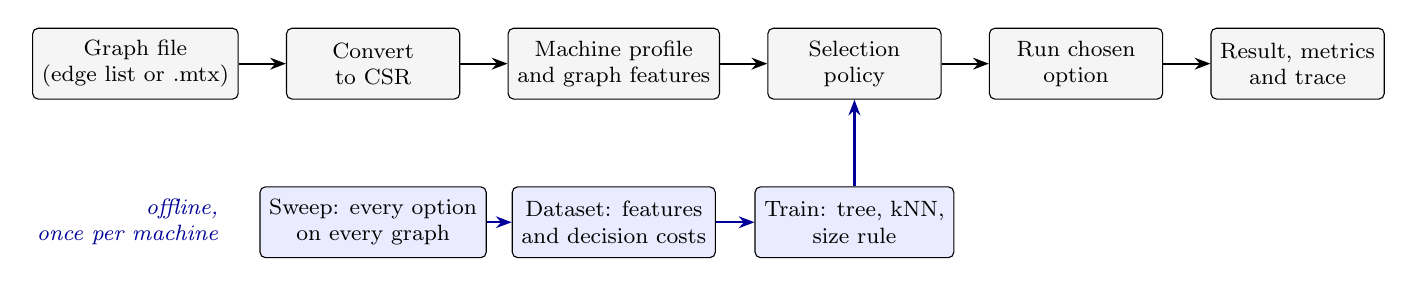
\begin{tikzpicture}[
  node distance=6mm,
  box/.style={draw, rounded corners=2pt, minimum height=9mm, minimum width=22mm, align=center, font=\footnotesize, fill=gray!8},
  off/.style={box, fill=blue!8},
  arr/.style={-{Stealth[length=2mm]}, thick}]
\node[box] (in) {Graph file\\(edge list or .mtx)};
\node[box, right=of in] (csr) {Convert\\to CSR};
\node[box, right=of csr] (feat) {Machine profile\\and graph features};
\node[box, right=of feat] (pol) {Selection\\policy};
\node[box, right=of pol] (run) {Run chosen\\option};
\node[box, right=of run] (out) {Result, metrics\\and trace};
\draw[arr] (in) -- (csr);
\draw[arr] (csr) -- (feat);
\draw[arr] (feat) -- (pol);
\draw[arr] (pol) -- (run);
\draw[arr] (run) -- (out);
\node[off, below=11mm of csr] (sweep) {Sweep: every option\\on every graph};
\node[off, below=11mm of feat] (data) {Dataset: features\\and decision costs};
\node[off, below=11mm of pol] (train) {Train: tree, kNN,\\size rule};
\draw[arr, blue!60!black] (sweep) -- (data);
\draw[arr, blue!60!black] (data) -- (train);
\draw[arr, blue!60!black] (train) -- (pol);
\node[font=\footnotesize\itshape, blue!60!black, left=4mm of sweep, align=right] {offline,\\once per machine};
\end{tikzpicture}
\caption{Pipeline. Top row: what happens for one query. Bottom row: the offline stage that produces the selection policy from measured runs. The machine profile removes CUDA from the option set when no GPU is present.}
\label{fig:pipeline}
\end{figure*}

%==============================================================
\section{Algorithms}
\subsection{Graph kernels}
Table~\ref{tab:alg} lists the formulations. Two rules guided the design. First, the algorithm is the same in every execution model, so that only the execution model changes; the single exception is connected components under MPI, where union-find does not distribute naturally and we use label propagation instead. Second, the parallel versions are deliberately vanilla (no tuning), because the baselines must stay a stable reference. OpenMP uses dynamic scheduling for loops over edges. The CUDA kernels assign one thread to each vertex or frontier vertex and use atomics. MPI splits the vertices into equal contiguous blocks and each rank owns the out-edges of its block; this partition is naive on purpose, so any imbalance on skewed graphs shows up in the results.

\begin{table}[t]
\caption{Kernel formulations. All models except MPI connected components use the same method.}
\label{tab:alg}
\centering\footnotesize
\begin{tabular}{@{}p{0.16\columnwidth}p{0.43\columnwidth}p{0.31\columnwidth}@{}}
\toprule
Kernel & Sequential, OpenMP, CUDA & MPI (vertex blocks) \\
\midrule
BFS & Level-synchronous frontier; vertices claimed by compare-and-swap & Remote discoveries exchanged by all-to-all each level \\
PageRank & Pull over transposed CSR; $d{=}0.85$, L1 tolerance $10^{-8}$, at most 100 iterations, dangling mass spread uniformly & Allgather of contributions; allreduce of residual \\
Conn. comp. & Union-find, larger root linked under smaller & Min-label propagation, allgather per round \\
SSSP & Frontier-based label-correcting; integer weights 1--100 & Relaxations sent to the owning rank \\
Triangles & Merge intersection of sorted neighbour lists, each triangle counted once & CSR replicated by allgather; each rank counts its block \\
\bottomrule
\end{tabular}
\end{table}

\subsection{Data layout and conventions}
Graphs are stored in compressed sparse row (CSR) form with 32-bit vertex ids and 64-bit offsets. The loader compacts vertex ids, removes self-loops and duplicate edges and sorts neighbour lists. Graphs are directed as loaded unless declared undirected. Connected components and triangle counting run on the symmetrized graph, so components are weakly connected components and triangles are counted on a simple undirected graph. SSSP weights are integers in $[1,100]$ derived from a hash of a fixed seed and the unordered endpoint pair, which makes them independent of vertex id, degree and edge order and identical across implementations.

\subsection{Selector algorithms}
Algorithm~\ref{alg:train} is run once per machine on the sweep data. Algorithm~\ref{alg:select} is run for every query.

\begin{algorithm}[t]
\caption{Offline training (once per machine)}\label{alg:train}
\begin{algorithmic}[1]
\Require decision costs $D_c(G,k)$ for all graphs $G$, kernels $k$ and measured options $c$; features $f(G)$
\Ensure one decision tree per kernel (full and CPU-only)
\For{each kernel $k$}
  \For{each graph $G$}
    \State $s_c \gets \ln(D_{\text{seq}}/D_c)$ for every measured option $c$
  \EndFor
  \State fit a depth-3 multi-output regression tree on $\{(f(G),s(G))\}$
  \State fit a second tree with CUDA removed (used without a GPU)
\EndFor
\State export the trees as JSON
\end{algorithmic}
\end{algorithm}

\begin{algorithm}[t]
\caption{Selection and execution of one query}\label{alg:select}
\begin{algorithmic}[1]
\Require graph file, kernel $k$
\State load the graph, build CSR, detect directedness
\State profile the machine; $\mathcal{C}\gets$ available options (CUDA only if a GPU is usable and the graph fits)
\State $f\gets$ six features (one pass over the vertices)
\State $\hat s_c\gets \text{tree}_k(f)$ for $c\in\mathcal{C}$ (CPU-only tree if CUDA $\notin\mathcal{C}$)
\State $c^\star\gets\arg\max_c \hat s_c$; if $\hat s_{c^\star}<\ln 1.05$ then $c^\star\gets$ sequential
\State run $c^\star$, validate, report compute time, end-to-end time and $T_{\text{sel}}$
\end{algorithmic}
\end{algorithm}

%==============================================================
\section{Experimental Setup}
\subsection{Graphs}
We use 34 graphs. Two are real SNAP graphs~\cite{snap}: ego-Facebook (4,039 vertices, 88,234 edges)~\cite{mcauley} and web-Google (875,713 vertices, 5,105,039 edges)~\cite{leskovec}. Our triangle count on web-Google, 13,391,903, matches the value published by SNAP. The other 32 are synthetic with fixed seeds: uniform random directed graphs, R-MAT graphs~\cite{rmat} (heavy-tailed degrees), small-world graphs~\cite{ws} and two-dimensional grids (long paths, equal degrees). Requested sizes run from $2^{10}$ to $2^{20}$ vertices, with mean degree 8 and, for some sizes, 2 or 32. Actual sizes are smaller than requested, because vertices without edges are dropped and duplicate edges removed; for example the R-MAT graph requested at $2^{20}$ vertices has 547,094. Degree skew (maximum over mean degree) ranges from 1.0 for grids to 1,544 for the largest R-MAT graph.

\subsection{Platforms}
\begin{table}[t]
\caption{Experimental platforms.}
\label{tab:platforms}
\centering\footnotesize
\begin{tabular}{@{}p{0.2\columnwidth}p{0.36\columnwidth}p{0.36\columnwidth}@{}}
\toprule
 & Mac (development) & Windows laptop (WSL2) \\
\midrule
CPU & \fillin{Apple chip}, 8 physical cores & \fillin{CPU model}, 16 logical processors visible \\
Memory & \fillin{RAM} & \fillin{RAM}; about 14\,GB visible to WSL2 \\
Accelerator & none & NVIDIA RTX 5090 (laptop) \\
OS & macOS \fillin{version} & Ubuntu \fillin{version} on WSL2 \\
Software & AppleClang 17, libomp (OpenMP 5.1) & \fillin{GCC version}, CUDA \fillin{12.8 or newer} \\
MPI & Open MPI \fillin{version} & Open MPI \fillin{version} \\
Workers swept & 1, 2, 4, 8 threads or ranks & 1, 2, 4, 8, 16 threads \\
\bottomrule
\end{tabular}
\end{table}
Table~\ref{tab:platforms} summarises the machines. The laptop was available for a limited time: its sequential, OpenMP and CUDA sweeps completed, but the MPI sweep aborted because Open MPI refused 16 ranks (by default it counts physical cores as slots and the run was not started with oversubscription). Only four MPI measurements exist for that machine, and they are excluded from every analysis. MPI results are therefore Mac-only, and since the laptop was returned before the demonstration, its GPU results are shown by replaying recorded data.

\subsection{Measurement protocol}
Each configuration has one untimed warm-up and three timed trials, and we report medians. OpenMP threads are pinned on Linux (\texttt{OMP\_PROC\_BIND=close}, \texttt{OMP\_PLACES=cores}); macOS offers no pinning. Every result row is appended to a tagged CSV that is never edited afterwards, results from different machines are never pooled, and each run stores its environment.

\subsection{Correctness validation}
Each trial-0 result is checked by an independent validator: BFS levels by a level-bound and parent check, SSSP by edge relaxation plus a tight predecessor for every reached vertex, components by partition equivalence against a flood fill, triangles by a separate edge-wise count, and PageRank by normalisation, convergence and an L1 distance of at most $10^{-7}$ to the sequential result. Unit tests compare against separate oracles (Bellman--Ford and Dijkstra for SSSP, brute-force triangle counting, a dense PageRank iteration) on random graphs with a hub vertex and on edge cases. All sweep runs on both machines passed validation.

\subsection{Selector evaluation}
We evaluate with leave-one-graph-out and leave-one-family-out splits (families: uniform, R-MAT, small-world, grid, and the two real graphs as their own families). Policies are trained without the held-out graph or family, and selection overhead is counted using the recorded feature-extraction time plus measured inference. The headline metric is total time over all instances divided by the oracle's total (the oracle picks the fastest option on every instance; 1.00 is perfect). We also report the share of instances slower than sequential, with differences below 0.1\,ms treated as ties. Totals are dominated by the longest runs, so per-instance behaviour is examined separately. The evaluation reuses the graphs on which design choices (the feature set, the guardrails) were made, so the numbers are optimistic to some degree.

%==============================================================
\section{Results}
\subsection{Raw runtimes}
Table~\ref{tab:raw} gives algorithm-only runtimes in seconds for three large graphs, with the fastest thread or rank count in parentheses. For CUDA we show the kernel time and, separately, the time including allocation and transfers.

\begin{table*}[t]
\caption{Algorithm-only runtimes in seconds (medians of three trials). Parentheses: thread or rank count of the fastest configuration. CUDA+xfer includes device allocation and host--device transfers.}
\label{tab:raw}
\centering\footnotesize
\safetable{tables/raw_runtimes.tex}
\end{table*}

\subsection{Speedups}
Figure~\ref{fig:speedup} shows speedup over the sequential run as a function of graph size on the laptop, and Table~\ref{tab:geomean} gives geometric-mean speedups over all 34 graphs.

\begin{figure*}[t]
\centering
\safefig{figs/fig_speedup_size.pdf}{0.78\textwidth}
\caption{Speedup over sequential versus graph size on the 5090 laptop (best configuration per graph; points are graphs, lines are binned medians; dashed: CUDA including transfers).}
\label{fig:speedup}
\end{figure*}

\begin{table}[t]
\caption{Geometric-mean speedup over sequential across all 34 graphs; best thread or rank count chosen per graph, so these are upper bounds for a fixed count.}
\label{tab:geomean}
\centering\footnotesize
\safetable{tables/geomean_speedup.tex}
\end{table}

\subsection{Fastest implementation and thread counts}
Table~\ref{tab:winners} counts how often each implementation was the fastest. OpenMP wins most instances on both machines, and MPI was fastest on one instance out of 170 on the Mac (PageRank on one graph). Sequential execution was fastest on 11 to 13 of the 34 graphs for BFS and on 6 to 14 for SSSP, depending on the machine, including some graphs between $2^{14}$ and $2^{20}$ vertices. Figure~\ref{fig:workers} shows the fastest OpenMP thread count: on the Mac, 4 threads won 47\% of instances (2 and 8 threads: 21\% and 32\%); on the laptop, 8 threads won 47\% and 16 threads 33\%. The GPU was fastest on 11 of 170 instances: SSSP (5), triangle counting (4), BFS (1) and PageRank (1).

\begin{table}[t]
\caption{Number of graphs (out of 34) on which each implementation was fastest by decision cost, among all measured configurations.}
\label{tab:winners}
\centering\footnotesize
\safetable{tables/winners.tex}
\end{table}

\begin{figure}[t]
\centering
\safefig{figs/fig_workers.pdf}{0.85\columnwidth}
\caption{Fastest OpenMP thread count per (graph, kernel) instance on each machine.}
\label{fig:workers}
\end{figure}

\subsection{GPU triangle counting and degree skew}
Table~\ref{tab:tc} shows triangle counting on the R-MAT graph with 547,094 vertices, where the CUDA kernel is slower than a single CPU thread. Across all graphs (Fig.~\ref{fig:skew}), every graph with degree skew of at most 3.1 that reached a 4$\times$ speedup or more was uniform or small-world, and all 12 graphs with skew of 24 or more, including both real graphs, stayed at or below 2.7$\times$; six of them were slower than sequential. No graph in our set has skew between 4.9 and 24.

\begin{table}[t]
\caption{Triangle counting on the R-MAT graph with 547,094 vertices (laptop): algorithm-only time and speedup over sequential. CUDA is kernel only.}
\label{tab:tc}
\centering\footnotesize
\begin{tabular}{@{}lrr@{}}
\toprule
Configuration & Time (s) & Speedup \\
\midrule
Sequential & 10.16 & 1.00 \\
OpenMP, 1 thread & 10.97 & 0.93 \\
OpenMP, 2 threads & 5.70 & 1.78 \\
OpenMP, 4 threads & 2.83 & 3.59 \\
OpenMP, 8 threads & 1.51 & 6.74 \\
OpenMP, 16 threads & 1.10 & 9.26 \\
CUDA (vanilla) & 14.34 & 0.71 \\
\bottomrule
\end{tabular}
\end{table}

\begin{figure}[t]
\centering
\safefig{figs/fig_cuda_skew.pdf}{0.85\columnwidth}
\caption{CUDA triangle-counting speedup (including transfers) versus degree skew, by graph family.}
\label{fig:skew}
\end{figure}

\subsection{Time breakdown}
Figure~\ref{fig:split} splits end-to-end time into its regions for the fastest option of each framework, on a large and a small graph.

\begin{figure*}[t]
\centering
\safefig{figs/fig_time_split.pdf}{0.85\textwidth}
\caption{Share of end-to-end time by region for the fastest option per framework (S: sequential, O: OpenMP, G: CUDA) on a large and a small synthetic graph, 5090 laptop.}
\label{fig:split}
\end{figure*}

\subsection{Selector}
Table~\ref{tab:selector} and Fig.~\ref{fig:selector} give total time on held-out inputs relative to the oracle in three scenarios: the Mac (CPU only), the laptop with CUDA removed from the options, and the laptop with the GPU.

\begin{table}[t]
\caption{Total time on held-out inputs relative to the oracle (1.00 = perfect), selection overhead included. In parentheses: percentage of instances slower than sequential.}
\label{tab:selector}
\centering\footnotesize
\begin{tabular}{@{}llrrrr@{}}
\toprule
Scenario & Held out & Seq. & Best fixed & Size rule & Tree \\
\midrule
Mac, CPU only & graph & 4.06 & 1.20 (5.3) & 1.09 (12.9) & \textbf{1.05} (7.1) \\
 & family & 4.06 & 1.20 (11.8) & 1.07 (13.5) & \textbf{1.05} (5.3) \\
5090, no GPU & graph & 7.72 & \textbf{1.05} (5.9) & 1.06 (4.1) & 1.07 (4.1) \\
 & family & 7.72 & \textbf{1.05} (5.9) & 1.06 (4.1) & 1.09 (5.9) \\
5090, GPU & graph & 8.96 & 1.21 (5.9) & 1.21 (3.5) & \textbf{1.08} (1.2) \\
 & family & 8.96 & \textbf{1.21} (5.9) & \textbf{1.21} (3.5) & 6.87 (5.3) \\
\bottomrule
\end{tabular}
\end{table}

\begin{figure*}[t]
\centering
\safefig{figs/fig_selector.pdf}{0.8\textwidth}
\caption{Total time relative to the oracle for four policies in three scenarios (selection overhead included; logarithmic axis).}
\label{fig:selector}
\end{figure*}

%==============================================================
\section{Performance Analysis}\label{sec:analysis}
\subsection{Scaling and the size threshold}
Parallel execution loses on small graphs because its fixed costs (thread start-up, synchronisation, message exchange, kernel launches and transfers) are not amortised. For connected components, PageRank and triangle counting the break-even lies at a few thousand vertices (the learned PageRank rule on the laptop switches at about 1.7 thousand). BFS and SSSP keep sequential execution competitive on a sizeable minority of graphs. A level-synchronous traversal pays a synchronisation on every level, so graphs with many levels and small frontiers are a plausible cause, but we did not isolate this. On the largest graphs scaling is good up to the physical core count and then flattens: triangle counting on the R-MAT graph reaches 3.6$\times$ with 4 OpenMP threads (90\% efficiency), 6.7$\times$ with 8 (84\%) and 9.3$\times$ with 16 (58\%); the last step uses hyperthreads on the laptop.

\subsection{Where the time goes}
Loading and preprocessing are the same for every option, so they set a floor under end-to-end time and dilute differences between frameworks. On the Mac, parsing and building the CSR for web-Google took about 1.6\,s and symmetrising it about 0.7\,s, while a BFS needs a few tens of milliseconds; the PageRank transpose took about 0.03\,s, roughly 3\% of the sequential PageRank run. Kernel time for the GPU excludes allocation and transfers, which is why Fig.~\ref{fig:speedup} shows both views: a GPU that is fast by kernel time can still lose in a one-shot run. MPI's setup includes distributing the graph through message passing. \fillin{check this subsection against Fig.~\ref{fig:split} once generated}

\subsection{Machine dependence}
OpenMP wins most instances on both machines, but the best thread count differs: 4 on the Mac and 8 or 16 on the laptop. The sweeps stop at 8 and 16 threads, so many winners sit at the top of the tested range and a higher count might have won. We expected the Mac's mix of performance and efficiency cores to play a role but did not verify it. A wrong choice between neighbouring thread counts is often cheap (R-MAT triangle counting takes 1.51\,s with 8 threads and 1.10\,s with 16), which is one reason a fixed choice is hard to beat on a single CPU. MPI was fastest once in 170 instances on the Mac. That is unsurprising on one node: MPI pays for distributing the graph through message passing and gains nothing from separate memories.

\subsection{GPU behaviour and degree skew}
The GPU wins only on large graphs and mostly for SSSP and triangle counting. Its failure on skewed graphs is the clearest result (Table~\ref{tab:tc}, Fig.~\ref{fig:skew}): the CUDA kernel is slower than one CPU thread while OpenMP scales almost linearly. We attribute this to load imbalance in the one-thread-per-vertex mapping, where a few hub vertices carry most of the work, but we have not profiled the kernel, so this remains a hypothesis. Skew, size and density rise together inside the R-MAT family, and the only other high-skew graphs are the two real ones, so the data are consistent with a skew effect but do not prove it. The empty range between skew 4.9 and 24 means we cannot say where the transition happens.

\subsection{Selector behaviour}
\emph{Selection helps when the choice is real.} On unseen graphs the tree stays within 5--8\% of the oracle in all three scenarios. On the Mac, where the best thread count varies by graph, it uses about 12\% less total time than the best fixed choice (1.05 against 1.20), and on the laptop with the GPU option about 11\% less (1.08 against 1.21). With the GPU, the tree also has the fewest instances slower than sequential (1.2\%).

\emph{It adds nothing on a CPU that scales smoothly.} On the laptop without the GPU the best fixed configuration is within 5\% of the oracle and the tree is slightly worse (1.07). A perfect selector with the GPU takes 14\% less total time than without it (0.112 against 0.130 of the sequential total), and the tree obtains 0.121.

\emph{Generalisation can fail badly.} With the R-MAT family held out, the tree's total time on the laptop is 6.87 times the oracle's, almost entirely from triangle counting on R-MAT graphs, where the tree chose CUDA. The training graphs for that fold contain nothing with skew above 78 or out-degree variation above 1.2, whereas the R-MAT graphs reach 1,544 and 6.9. The learned rule is effectively ``large, dense, non-grid graph: use CUDA''. It is right on the training graphs and wrong on the most skewed ones, where the vanilla kernel is slower than sequential. The size rule never chose CUDA and was unaffected (1.21). The failure comes from the training set not covering that part of the feature space and the model having no basis to extrapolate.

\emph{The two learned models trade accuracy for cost.} kNN had the highest rate of picking a near-best option (about 81\% on unseen graphs with the GPU), but its pure-Python inference made selection overhead average roughly 40\% of an instance's time, so it is not our headline model. For the tree the average overhead is 20--25\%, because many graphs are so small that a run takes microseconds and feature extraction already costs more than selection could save. The selector therefore pays off only above a break-even size; skipping selection for tiny graphs is an obvious refinement that we have not evaluated.

%==============================================================
\section{Comparison with Existing Methods}
\subsection{Against default policies}
The practitioner's alternatives to a selector are in Table~\ref{tab:selector}. ``Always sequential'' is what a user does without parallel code and costs 4 to 9 times the oracle. ``Best fixed'' is a configuration tuned once per machine, which is common practice, and the size rule is a rule of thumb fitted to the same data. Compared with the best fixed choice the tree saves about 12\% of total time on the Mac and 11\% on the laptop with the GPU, is equal or slightly worse on the laptop CPU, and loses badly on the unseen R-MAT family. Compared with exhaustive per-instance measurement, which is what the oracle represents, the tree needs one pass over the vertices and a tree lookup, whereas measuring would have to run nine (Mac) or seven (laptop) configurations each time.

\subsection{Against published systems and autotuners}
We did not run external frameworks, so Table~\ref{tab:compare} is a qualitative comparison of what each approach decides, when, and at what cost. It is not a performance comparison with published systems. The only external check on correctness is the triangle count on web-Google, which matches the value published by SNAP.

\begin{table}[t]
\caption{Qualitative comparison with existing approaches. None of the published systems was run.}
\label{tab:compare}
\centering\footnotesize
\begin{tabular}{@{}p{0.2\columnwidth}p{0.17\columnwidth}p{0.17\columnwidth}p{0.3\columnwidth}@{}}
\toprule
Approach & Decides & When & Cost of deciding \\
\midrule
Fixed configuration (hand tuned) & one setup per machine & once & none per run \\
Empirical autotuning~\cite{atlas,fftw} & implementation and parameters & install or planning time & runs the candidates \\
Switching inside an algorithm~\cite{dobfs,ligra} & traversal direction & during the run & per-level frontier statistics \\
Scheduling languages~\cite{graphit} & schedule & compile time & manual or searched \\
This work & execution model and worker count & before the run & one pass over the vertices and a tree lookup \\
\bottomrule
\end{tabular}
\end{table}

%==============================================================
\section{Limitations and Threats to Validity}
\begin{itemize}
\item One machine per scenario, and the laptop runs under WSL2 with hyperthreads, a mobile GPU and a power state we did not control precisely.
\item Three trials per configuration; medians are stable but intervals are coarse.
\item MPI is single-node and the laptop's MPI sweep did not complete, so MPI conclusions come from the Mac only.
\item The CUDA kernels are vanilla. GPU results describe an untuned implementation, not the potential of the hardware.
\item Thirty-two of the 34 graphs come from four generators, and each real family has one graph, so structural conclusions are limited.
\item Features describe the graph as loaded, while connected components and triangle counting run on the symmetrized graph.
\item Feature choices and guardrails were designed after looking at evaluation results on the same graphs; leave-one-out evaluation only partly protects against this.
\item Selectors are trained per machine and cannot transfer to new hardware.
\end{itemize}

%==============================================================
\section{Conclusion}
We built and measured five graph kernels in four execution models on two machines, and used the measurements to train a small selector. The baselines show a size threshold for parallelism, machine-dependent thread counts, a GPU that wins only on large, low-skew inputs, and run times in which loading, preprocessing and data movement matter. The selector pays for its own overhead and saves about 11--13\% of total time over the best fixed choice where there is a real choice, but not on a smoothly scaling CPU, and it breaks outside the range of structures it was trained on.

%==============================================================
\section{Future Scope}
The failures point to the next steps: profile the CUDA triangle-counting kernel and fix its load balance, add cheap structure features such as a diameter estimate, and cover more graph families and machines. Beyond that: collect multi-node MPI data, evaluate skipping selection for tiny graphs, add hardware microbenchmark features so a selector can generalise to unseen machines, and build the mid-run switching classifier and tuned GPU variants originally planned for this project. A systematic survey of learned selection for graph systems should precede any novelty claim.

%==============================================================
\begin{thebibliography}{99}
\bibitem{gap} S. Beamer, K. Asanovi\'c, and D. Patterson, ``The GAP benchmark suite,'' arXiv:1508.03619, 2015.
\bibitem{lumsdaine} A. Lumsdaine, D. Gregor, B. Hendrickson, and J. Berry, ``Challenges in parallel graph processing,'' \emph{Parallel Processing Letters}, vol. 17, no. 1, 2007.
\bibitem{pregel} G. Malewicz et al., ``Pregel: A system for large-scale graph processing,'' in \emph{Proc. ACM SIGMOD}, 2010.
\bibitem{ligra} J. Shun and G. E. Blelloch, ``Ligra: A lightweight graph processing framework for shared memory,'' in \emph{Proc. ACM PPoPP}, 2013.
\bibitem{galois} D. Nguyen, A. Lenharth, and K. Pingali, ``A lightweight infrastructure for graph analytics,'' in \emph{Proc. ACM SOSP}, 2013.
\bibitem{gunrock} Y. Wang et al., ``Gunrock: A high-performance graph processing library on the GPU,'' in \emph{Proc. ACM PPoPP}, 2016.
\bibitem{merrill} D. Merrill, M. Garland, and A. Grimshaw, ``Scalable GPU graph traversal,'' in \emph{Proc. ACM PPoPP}, 2012.
\bibitem{graphit} Y. Zhang et al., ``GraphIt: A high-performance graph DSL,'' \emph{Proc. ACM Program. Lang.} (OOPSLA), 2018.
\bibitem{dobfs} S. Beamer, K. Asanovi\'c, and D. Patterson, ``Direction-optimizing breadth-first search,'' in \emph{Proc. SC}, 2012.
\bibitem{sv} Y. Shiloach and U. Vishkin, ``An $O(\log n)$ parallel connectivity algorithm,'' \emph{J. Algorithms}, vol. 3, no. 1, 1982.
\bibitem{delta} U. Meyer and P. Sanders, ``$\Delta$-stepping: A parallelizable shortest path algorithm,'' \emph{J. Algorithms}, vol. 49, no. 1, 2003.
\bibitem{rice} J. R. Rice, ``The algorithm selection problem,'' \emph{Advances in Computers}, vol. 15, 1976.
\bibitem{atlas} R. C. Whaley, A. Petitet, and J. J. Dongarra, ``Automated empirical optimization of software and the ATLAS project,'' \emph{Parallel Computing}, vol. 27, 2001.
\bibitem{fftw} M. Frigo and S. G. Johnson, ``The design and implementation of FFTW3,'' \emph{Proc. IEEE}, vol. 93, no. 2, 2005.
\bibitem{snap} J. Leskovec and A. Krevl, ``SNAP Datasets: Stanford large network dataset collection,'' 2014. [Online]. Available: http://snap.stanford.edu/data
\bibitem{mcauley} J. McAuley and J. Leskovec, ``Learning to discover social circles in ego networks,'' in \emph{Proc. NIPS}, 2012.
\bibitem{leskovec} J. Leskovec, K. Lang, A. Dasgupta, and M. Mahoney, ``Community structure in large networks,'' \emph{Internet Mathematics}, vol. 6, no. 1, 2009.
\bibitem{rmat} D. Chakrabarti, Y. Zhan, and C. Faloutsos, ``R-MAT: A recursive model for graph mining,'' in \emph{Proc. SIAM SDM}, 2004.
\bibitem{ws} D. J. Watts and S. H. Strogatz, ``Collective dynamics of `small-world' networks,'' \emph{Nature}, vol. 393, 1998.
\bibitem{cart} L. Breiman, J. Friedman, R. Olshen, and C. Stone, \emph{Classification and Regression Trees}. Wadsworth, 1984.
\bibitem{knn} T. Cover and P. Hart, ``Nearest neighbor pattern classification,'' \emph{IEEE Trans. Inf. Theory}, vol. 13, no. 1, 1967.
\bibitem{sklearn} F. Pedregosa et al., ``Scikit-learn: Machine learning in Python,'' \emph{J. Mach. Learn. Res.}, vol. 12, 2011.
\end{thebibliography}

\end{document}\documentclass[conference]{IEEEtran}
\usepackage{cite}
\usepackage{amsmath,amssymb}
\usepackage{graphicx}
\usepackage{booktabs}
\usepackage{xcolor}
\usepackage{tikz}
\usetikzlibrary{arrows.meta,positioning}
\usepackage{algorithm}
\usepackage{algpseudocode}
\usepackage{url}
\newcommand{\fillin}[1]{\textcolor{red}{[#1]}}
\newcommand{\safefig}[2]{\IfFileExists{#1}{\includegraphics[width=#2]{#1}}{\fbox{\parbox{#2}{\centering\footnotesize figure missing}}}}
\newcommand{\safetable}[1]{\IfFileExists{#1}{\input{#1}}{\fillin{missing table; run make\_report\_tables.py}}}

\begin{document}

\title{Choosing How to Run Graph Algorithms:\\
Sequential, OpenMP, MPI and CUDA Baselines\\
and a Lightweight Execution Selector}

\author{\IEEEauthorblockN{\fillin{Author 1}, \fillin{Author 2}, \fillin{Author 3}}
\IEEEauthorblockA{\fillin{Department, University}\\
Course project report, November 2026}}

\maketitle

\begin{abstract}
Graph algorithms rarely behave the same way across hardware, graph structures and execution models. We implement five kernels (BFS, PageRank, connected components, single-source shortest paths and triangle counting) in four vanilla execution models (sequential, OpenMP, single-node MPI and CUDA) and measure them on 34 graphs, two real and 32 synthetic, on two machines: an Apple Silicon laptop and a Windows laptop (WSL2) with an RTX 5090. Every run is validated by an independent checker, and timing is split into loading, preprocessing, setup, transfers, communication and compute. We find that parallelism pays off above a modest size threshold, that the best thread count differs between the two machines, that the GPU wins only on the largest and least skewed inputs, and that loading, preprocessing and data movement often decide end-to-end time. From these measurements we train a lightweight selector that picks an implementation and worker count from six cheap graph features. With its own overhead counted, a decision tree finishes within 5--8\% of an oracle on unseen graphs and uses about 11--13\% less total time than the best fixed choice when the choice is non-trivial. It gives no gain on a CPU-only machine, where a fixed choice is nearly optimal, and it fails on an unseen graph family. We describe two guardrails and the limits of the study.
\end{abstract}

\begin{IEEEkeywords}
graph analytics, OpenMP, MPI, CUDA, performance evaluation, algorithm selection
\end{IEEEkeywords}

%==============================================================
\section{Introduction}
Graph algorithms sit underneath web search, social network analysis, recommendation and a growing share of scientific computing. How fast they run depends on at least four things at once: the algorithm, the structure of the graph, the memory behaviour of the implementation and the hardware underneath. Parallel execution does not help uniformly. A kernel that scales well on a million-vertex graph can be slower than a single thread on a thousand-vertex one, a GPU can lose to one CPU core on a graph with very uneven degrees, and the work around an algorithm (loading, preprocessing, copying data to a device, exchanging messages) can cost more than the algorithm itself.

In practice someone has to choose between a sequential, multicore, distributed or GPU implementation for every job, and the right answer changes with the input and the machine. Rules of thumb exist, but we found few quantitative, reproducible comparisons that put all four execution models on the same graphs under one timing definition and then ask whether the choice can be automated cheaply. That gap motivates this work.

This paper does two things. It builds and measures a controlled baseline of five kernels in four execution models, and it uses those measurements to train a small selector that is judged honestly: with its own overhead counted, and on graphs and graph families it has not seen. Our contributions are a reproducible measurement framework with independent correctness checks; a baseline study of 34 graphs on two machines (2,720 configuration measurements, three trials each); a lightweight selector evaluated against fixed and rule-based policies, with two guardrails and a command-line and web interface; and an account of where the selector fails. This is a course project. MPI runs on a single node, the CUDA kernels are deliberately untuned, and we make no novelty claim (Section~\ref{sec:related}).

%==============================================================
\section{Literature Review}\label{sec:related}
\textit{Benchmarks and suites.} The GAP Benchmark Suite~\cite{gap} defines a small set of kernels, including BFS, SSSP, PageRank, connected components and triangle counting, and a methodology for comparing implementations. We borrow its kernel set and its insistence on stating exactly what is timed. Lumsdaine et al.~\cite{lumsdaine} explain why irregular memory access and skewed degree distributions make these problems hard to scale.

\textit{Frameworks.} Pregel~\cite{pregel} popularised vertex-centric distributed processing. Ligra~\cite{ligra} and Galois~\cite{galois} target shared memory, while Gunrock~\cite{gunrock} and the GPU traversal work of Merrill et al.~\cite{merrill} target GPUs. GraphIt~\cite{graphit} separates an algorithm from its schedule. These systems expose choices such as push versus pull and sparse versus dense frontiers, which are normally tuned by hand or by search.

\textit{Switching within an algorithm.} Direction-optimizing BFS~\cite{dobfs} alternates between top-down and bottom-up traversal depending on the frontier, and Ligra applies a similar idea. This is a within-run choice inside one algorithm. Our selector works at a coarser level, one decision per run across execution models. Switching strategies during a run is left for future work.

\textit{Kernel formulations.} Our connected-components kernel follows the union-find tradition, with Shiloach--Vishkin~\cite{sv} as the classical parallel alternative. Our SSSP kernel is a frontier-based label-correcting method; $\Delta$-stepping~\cite{delta} is the natural next step.

\textit{Algorithm and implementation selection.} Rice~\cite{rice} formalised the algorithm selection problem. Empirical autotuners such as ATLAS~\cite{atlas} and FFTW~\cite{fftw} choose among implementations by measuring them on the target machine; a learned selector replaces part of that measurement with a model. We did not survey learned selection for graph systems systematically, so we claim no novelty. What this paper contributes is a small, fully reproducible case study that counts selection overhead and tests on unseen graph families.

%==============================================================
\section{Problem Statement}
Let $G$ be an input graph, $k$ one of five kernels, and $M$ a machine whose available options $\mathcal{C}_M$ are the sequential run, OpenMP and MPI at several worker counts, and CUDA when a GPU is present. Running option $c$ costs $D_c(G,k,M)$ (Eq.~\ref{eq:dc}) on top of loading and preprocessing, which are common to all options. The problem has two parts.

\emph{Characterisation.} How does $D_c$ vary with graph size, structure, kernel and machine, and which parts of a run (setup, transfers, communication, compute) dominate?

\emph{Selection.} Find a policy $\pi$ that maps cheap features of $G$ and the kernel to an option so that the realised cost $T_\pi = D_{\pi}+T_{\text{sel}}$, including the selector's own overhead $T_{\text{sel}}$, is close to the oracle's $\min_c D_c$ on graphs and graph families not used for training.

The problem is constrained: only a few dozen graphs are available per machine, selection must cost much less than a run, results must be correct, and nothing beyond the two machines at hand can be assumed.

%==============================================================
\section{Objectives}
\begin{enumerate}
\item Implement five kernels in four execution models on a shared CSR representation, keeping the algorithm fixed across models so that only the execution model changes.
\item Define one timing contract and independent correctness checks, and measure every option on 34 graphs on two machines.
\item Characterise when each model pays off and where the time goes.
\item Learn a lightweight selector from the measurements and evaluate it against fixed and rule-based policies on held-out graphs and families, with its overhead counted.
\item Add guardrails for missing hardware and out-of-range inputs, and provide a usable command-line and web interface.
\item Report limits and negative results alongside the successes.
\end{enumerate}

%==============================================================
\section{Proposed Methodology}
The method has two stages (Fig.~\ref{fig:pipeline}). In the \emph{measurement stage} every option is run on every graph under a common timing contract, which produces a table of decision costs. In the \emph{selection stage} a small model maps six graph features to predicted speedups and the best available option is run.

\subsection{Timing contract and decision cost}
Every run records separate regions: loading ($T_{\text{load}}$), preprocessing ($T_{\text{prep}}$: transposing, symmetrizing or generating weights), setup (MPI graph distribution; CUDA allocation and graph upload), compute, MPI communication, device-to-host copies and end-to-end time. Compute is the algorithm call for sequential and OpenMP, CUDA events around the kernels for CUDA (so it excludes transfers), and the maximum over ranks including communication for MPI. Compute-only and end-to-end figures are never compared with each other. Because loading and preprocessing are identical for every option, the part of a run that depends on the choice is the \emph{decision cost}
\begin{equation}
D_c = T^{\text{e2e}}_c - T_{\text{load}} - T_{\text{prep}},\label{eq:dc}
\end{equation}
which is what the selector tries to minimise.

\subsection{Selection target}
For option $c$ the target is the log speedup over sequential, $s_c=\ln(D_{\text{seq}}/D_c)$. The model predicts $s_c$ for every available option and the selector picks the largest. Predicting a ratio removes the effect of graph scale, and because $D_{\text{seq}}$ is common to all options it cancels in the argmax. If no option is predicted to beat 1.05$\times$, the selector stays sequential. A policy's realised cost is $T_\pi = D_{\pi}+T_{\text{sel}}$.

\subsection{Features}
Six features describe the graph: $\log_{10}n$, $\log_{10}(1+\text{mean degree})$, $\log_{10}(1+\text{degree skew})$, the coefficient of variation of the out-degree, the fraction of dangling vertices and a symmetry flag. All come from the CSR row pointers in one pass over the vertices. This restriction matters. Our first version also computed in-degree statistics and checked symmetry, which cost a pass over every edge, as much as a BFS; on the Mac the selection overhead then averaged roughly 51--58\% of an instance's policy time. Hardware features (core counts, bandwidths) are not used: with two machines they would only identify the machine, so we train one selector per machine.

\subsection{Policies, and why these two models}
We compare five policies: always sequential, the single best fixed configuration, a size-threshold rule fitted to the training graphs, a $k$-nearest-neighbour model ($k{=}3$, standardised features, similarity-weighted average of neighbours' $s_c$) and a decision tree (CART~\cite{cart} as implemented in scikit-learn~\cite{sklearn}, multi-output regression of all $s_c$, depth 3, at least three graphs per leaf). The tree is exported as plain JSON so that inference needs no machine-learning library.

We chose a tree and a nearest-neighbour model for the same reasons. With 34 graphs per kernel on a machine, heavier models such as forests, boosting or neural networks would overfit and would add inference time that our own metric charges for. Both are cheap to evaluate and need no tuning beyond one or two integers. They are also complementary: nearest neighbours~\cite{knn} give a local, instance-based answer and a tree gives global thresholds that read as rules (``below roughly 1.7 thousand vertices stay sequential; above $6.9\times10^{5}$ vertices run SSSP on the GPU''). Readable rules were important because the decisions had to be explainable in a demonstration. The size rule is a sanity baseline: if a learned model cannot beat a single threshold, the extra machinery is not justified.

\subsection{Guardrails}
\textit{No GPU.} All policies see, and choose among, only the options that exist on the machine. When no GPU is detected CUDA is removed from the option set, from the training data and from the oracle, a separate CPU-only tree is exported next to the full one, and the comparison tables list CUDA explicitly as excluded instead of silently dropping it. A model trained on another machine therefore still produces a valid decision, although its CPU behaviour reflects the machine it was trained on.

\textit{Out-of-range inputs.} % keep this paragraph only if the warning edits are applied to gps.py, replay.py and app.py
The selector can report when a graph's features lie outside the training range. We added this after observing a failure (Section~\ref{sec:analysis}) and checked it on the same data. It fires on 95 of 170 held-out-family instances (56\%) and does not separate bad choices from good ones (11 of 18 costly picks versus 84 of 152 others, with the comparison including selection overhead), so we present it as a coverage notice, not a failure detector.

%==============================================================
\section{System Architecture}
Figure~\ref{fig:pipeline} shows the pipeline. The code is organised in layers. A shared core holds the CSR structure, the loader, feature extraction, validators and the timing and record code. Four implementation libraries (sequential, OpenMP, MPI, CUDA) implement the five kernels against that core, and three driver programs run them: one for sequential and OpenMP, one launched under \texttt{mpirun}, and one for CUDA. Each driver appends one CSV row per trial. Benchmark scripts sweep thread and rank counts over a registry of graphs (a manifest with family and directedness) and record the environment. Analysis scripts turn raw rows into tables and figures. The selector layer reads the sweep to build the training table, trains and evaluates policies, and serves decisions through a command-line tool, a web page and a replay mode. Unit tests with independent oracles guard every implementation. Raw results are append-only and tagged, graphs are generated from seeds listed in the manifest, and each run stores the environment (commit, CPU, compiler, driver).

\textit{Tooling.} The command-line tool takes a graph and a kernel, detects format and directedness, converts the graph to CSR, profiles the machine, extracts features, chooses an option, runs it and prints a trace with raw compute time, end-to-end time and selection overhead. A small web page wraps the same tool (file upload and a kernel dropdown). Because the GPU laptop was available only for the sweep, a replay mode runs the selector on recorded measurements; every time it prints is a recorded measurement and the output is labelled as a replay.

\begin{figure*}[t]
\centering
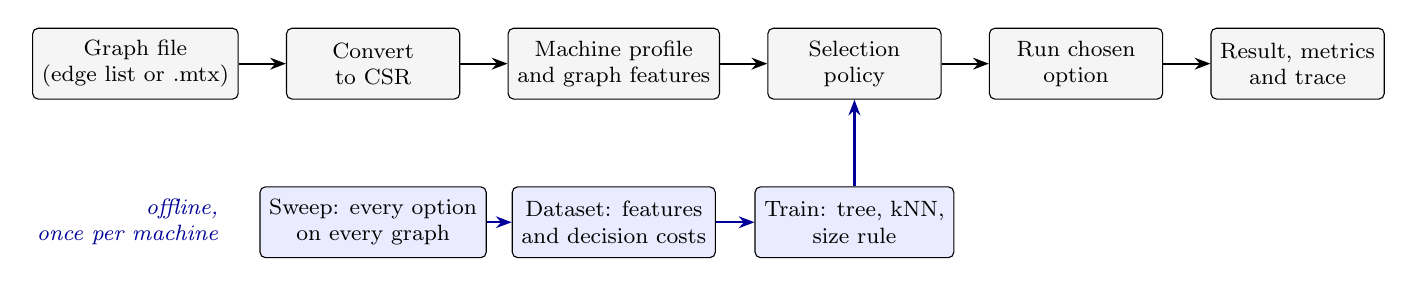
\begin{tikzpicture}[
  node distance=6mm,
  box/.style={draw, rounded corners=2pt, minimum height=9mm, minimum width=22mm, align=center, font=\footnotesize, fill=gray!8},
  off/.style={box, fill=blue!8},
  arr/.style={-{Stealth[length=2mm]}, thick}]
\node[box] (in) {Graph file\\(edge list or .mtx)};
\node[box, right=of in] (csr) {Convert\\to CSR};
\node[box, right=of csr] (feat) {Machine profile\\and graph features};
\node[box, right=of feat] (pol) {Selection\\policy};
\node[box, right=of pol] (run) {Run chosen\\option};
\node[box, right=of run] (out) {Result, metrics\\and trace};
\draw[arr] (in) -- (csr);
\draw[arr] (csr) -- (feat);
\draw[arr] (feat) -- (pol);
\draw[arr] (pol) -- (run);
\draw[arr] (run) -- (out);
\node[off, below=11mm of csr] (sweep) {Sweep: every option\\on every graph};
\node[off, below=11mm of feat] (data) {Dataset: features\\and decision costs};
\node[off, below=11mm of pol] (train) {Train: tree, kNN,\\size rule};
\draw[arr, blue!60!black] (sweep) -- (data);
\draw[arr, blue!60!black] (data) -- (train);
\draw[arr, blue!60!black] (train) -- (pol);
\node[font=\footnotesize\itshape, blue!60!black, left=4mm of sweep, align=right] {offline,\\once per machine};
\end{tikzpicture}
\caption{Pipeline. Top row: what happens for one query. Bottom row: the offline stage that produces the selection policy from measured runs. The machine profile removes CUDA from the option set when no GPU is present.}
\label{fig:pipeline}
\end{figure*}

%==============================================================
\section{Algorithms}
\subsection{Graph kernels}
Table~\ref{tab:alg} lists the formulations. Two rules guided the design. First, the algorithm is the same in every execution model, so that only the execution model changes; the single exception is connected components under MPI, where union-find does not distribute naturally and we use label propagation instead. Second, the parallel versions are deliberately vanilla (no tuning), because the baselines must stay a stable reference. OpenMP uses dynamic scheduling for loops over edges. The CUDA kernels assign one thread to each vertex or frontier vertex and use atomics. MPI splits the vertices into equal contiguous blocks and each rank owns the out-edges of its block; this partition is naive on purpose, so any imbalance on skewed graphs shows up in the results.

\begin{table}[t]
\caption{Kernel formulations. All models except MPI connected components use the same method.}
\label{tab:alg}
\centering\footnotesize
\begin{tabular}{@{}p{0.16\columnwidth}p{0.43\columnwidth}p{0.31\columnwidth}@{}}
\toprule
Kernel & Sequential, OpenMP, CUDA & MPI (vertex blocks) \\
\midrule
BFS & Level-synchronous frontier; vertices claimed by compare-and-swap & Remote discoveries exchanged by all-to-all each level \\
PageRank & Pull over transposed CSR; $d{=}0.85$, L1 tolerance $10^{-8}$, at most 100 iterations, dangling mass spread uniformly & Allgather of contributions; allreduce of residual \\
Conn. comp. & Union-find, larger root linked under smaller & Min-label propagation, allgather per round \\
SSSP & Frontier-based label-correcting; integer weights 1--100 & Relaxations sent to the owning rank \\
Triangles & Merge intersection of sorted neighbour lists, each triangle counted once & CSR replicated by allgather; each rank counts its block \\
\bottomrule
\end{tabular}
\end{table}

\subsection{Data layout and conventions}
Graphs are stored in compressed sparse row (CSR) form with 32-bit vertex ids and 64-bit offsets. The loader compacts vertex ids, removes self-loops and duplicate edges and sorts neighbour lists. Graphs are directed as loaded unless declared undirected. Connected components and triangle counting run on the symmetrized graph, so components are weakly connected components and triangles are counted on a simple undirected graph. SSSP weights are integers in $[1,100]$ derived from a hash of a fixed seed and the unordered endpoint pair, which makes them independent of vertex id, degree and edge order and identical across implementations.

\subsection{Selector algorithms}
Algorithm~\ref{alg:train} is run once per machine on the sweep data. Algorithm~\ref{alg:select} is run for every query.

\begin{algorithm}[t]
\caption{Offline training (once per machine)}\label{alg:train}
\begin{algorithmic}[1]
\Require decision costs $D_c(G,k)$ for all graphs $G$, kernels $k$ and measured options $c$; features $f(G)$
\Ensure one decision tree per kernel (full and CPU-only)
\For{each kernel $k$}
  \For{each graph $G$}
    \State $s_c \gets \ln(D_{\text{seq}}/D_c)$ for every measured option $c$
  \EndFor
  \State fit a depth-3 multi-output regression tree on $\{(f(G),s(G))\}$
  \State fit a second tree with CUDA removed (used without a GPU)
\EndFor
\State export the trees as JSON
\end{algorithmic}
\end{algorithm}

\begin{algorithm}[t]
\caption{Selection and execution of one query}\label{alg:select}
\begin{algorithmic}[1]
\Require graph file, kernel $k$
\State load the graph, build CSR, detect directedness
\State profile the machine; $\mathcal{C}\gets$ available options (CUDA only if a GPU is usable and the graph fits)
\State $f\gets$ six features (one pass over the vertices)
\State $\hat s_c\gets \text{tree}_k(f)$ for $c\in\mathcal{C}$ (CPU-only tree if CUDA $\notin\mathcal{C}$)
\State $c^\star\gets\arg\max_c \hat s_c$; if $\hat s_{c^\star}<\ln 1.05$ then $c^\star\gets$ sequential
\State run $c^\star$, validate, report compute time, end-to-end time and $T_{\text{sel}}$
\end{algorithmic}
\end{algorithm}

%==============================================================
\section{Experimental Setup}
\subsection{Graphs}
We use 34 graphs. Two are real SNAP graphs~\cite{snap}: ego-Facebook (4,039 vertices, 88,234 edges)~\cite{mcauley} and web-Google (875,713 vertices, 5,105,039 edges)~\cite{leskovec}. Our triangle count on web-Google, 13,391,903, matches the value published by SNAP. The other 32 are synthetic with fixed seeds: uniform random directed graphs, R-MAT graphs~\cite{rmat} (heavy-tailed degrees), small-world graphs~\cite{ws} and two-dimensional grids (long paths, equal degrees). Requested sizes run from $2^{10}$ to $2^{20}$ vertices, with mean degree 8 and, for some sizes, 2 or 32. Actual sizes are smaller than requested, because vertices without edges are dropped and duplicate edges removed; for example the R-MAT graph requested at $2^{20}$ vertices has 547,094. Degree skew (maximum over mean degree) ranges from 1.0 for grids to 1,544 for the largest R-MAT graph.

\subsection{Platforms}
\begin{table}[t]
\caption{Experimental platforms.}
\label{tab:platforms}
\centering\footnotesize
\begin{tabular}{@{}p{0.2\columnwidth}p{0.36\columnwidth}p{0.36\columnwidth}@{}}
\toprule
 & Mac (development) & Windows laptop (WSL2) \\
\midrule
CPU & \fillin{Apple chip}, 8 physical cores & \fillin{CPU model}, 16 logical processors visible \\
Memory & \fillin{RAM} & \fillin{RAM}; about 14\,GB visible to WSL2 \\
Accelerator & none & NVIDIA RTX 5090 (laptop) \\
OS & macOS \fillin{version} & Ubuntu \fillin{version} on WSL2 \\
Software & AppleClang 17, libomp (OpenMP 5.1) & \fillin{GCC version}, CUDA \fillin{12.8 or newer} \\
MPI & Open MPI \fillin{version} & Open MPI \fillin{version} \\
Workers swept & 1, 2, 4, 8 threads or ranks & 1, 2, 4, 8, 16 threads \\
\bottomrule
\end{tabular}
\end{table}
Table~\ref{tab:platforms} summarises the machines. The laptop was available for a limited time: its sequential, OpenMP and CUDA sweeps completed, but the MPI sweep aborted because Open MPI refused 16 ranks (by default it counts physical cores as slots and the run was not started with oversubscription). Only four MPI measurements exist for that machine, and they are excluded from every analysis. MPI results are therefore Mac-only, and since the laptop was returned before the demonstration, its GPU results are shown by replaying recorded data.

\subsection{Measurement protocol}
Each configuration has one untimed warm-up and three timed trials, and we report medians. OpenMP threads are pinned on Linux (\texttt{OMP\_PROC\_BIND=close}, \texttt{OMP\_PLACES=cores}); macOS offers no pinning. Every result row is appended to a tagged CSV that is never edited afterwards, results from different machines are never pooled, and each run stores its environment.

\subsection{Correctness validation}
Each trial-0 result is checked by an independent validator: BFS levels by a level-bound and parent check, SSSP by edge relaxation plus a tight predecessor for every reached vertex, components by partition equivalence against a flood fill, triangles by a separate edge-wise count, and PageRank by normalisation, convergence and an L1 distance of at most $10^{-7}$ to the sequential result. Unit tests compare against separate oracles (Bellman--Ford and Dijkstra for SSSP, brute-force triangle counting, a dense PageRank iteration) on random graphs with a hub vertex and on edge cases. All sweep runs on both machines passed validation.

\subsection{Selector evaluation}
We evaluate with leave-one-graph-out and leave-one-family-out splits (families: uniform, R-MAT, small-world, grid, and the two real graphs as their own families). Policies are trained without the held-out graph or family, and selection overhead is counted using the recorded feature-extraction time plus measured inference. The headline metric is total time over all instances divided by the oracle's total (the oracle picks the fastest option on every instance; 1.00 is perfect). We also report the share of instances slower than sequential, with differences below 0.1\,ms treated as ties. Totals are dominated by the longest runs, so per-instance behaviour is examined separately. The evaluation reuses the graphs on which design choices (the feature set, the guardrails) were made, so the numbers are optimistic to some degree.

%==============================================================
\section{Results}
\subsection{Raw runtimes}
Table~\ref{tab:raw} gives algorithm-only runtimes in seconds for three large graphs, with the fastest thread or rank count in parentheses. For CUDA we show the kernel time and, separately, the time including allocation and transfers.

\begin{table*}[t]
\caption{Algorithm-only runtimes in seconds (medians of three trials). Parentheses: thread or rank count of the fastest configuration. CUDA+xfer includes device allocation and host--device transfers.}
\label{tab:raw}
\centering\footnotesize
\safetable{tables/raw_runtimes.tex}
\end{table*}

\subsection{Speedups}
Figure~\ref{fig:speedup} shows speedup over the sequential run as a function of graph size on the laptop, and Table~\ref{tab:geomean} gives geometric-mean speedups over all 34 graphs.

\begin{figure*}[t]
\centering
\safefig{figs/fig_speedup_size.pdf}{0.78\textwidth}
\caption{Speedup over sequential versus graph size on the 5090 laptop (best configuration per graph; points are graphs, lines are binned medians; dashed: CUDA including transfers).}
\label{fig:speedup}
\end{figure*}

\begin{table}[t]
\caption{Geometric-mean speedup over sequential across all 34 graphs; best thread or rank count chosen per graph, so these are upper bounds for a fixed count.}
\label{tab:geomean}
\centering\footnotesize
\safetable{tables/geomean_speedup.tex}
\end{table}

\subsection{Fastest implementation and thread counts}
Table~\ref{tab:winners} counts how often each implementation was the fastest. OpenMP wins most instances on both machines, and MPI was fastest on one instance out of 170 on the Mac (PageRank on one graph). Sequential execution was fastest on 11 to 13 of the 34 graphs for BFS and on 6 to 14 for SSSP, depending on the machine, including some graphs between $2^{14}$ and $2^{20}$ vertices. Figure~\ref{fig:workers} shows the fastest OpenMP thread count: on the Mac, 4 threads won 47\% of instances (2 and 8 threads: 21\% and 32\%); on the laptop, 8 threads won 47\% and 16 threads 33\%. The GPU was fastest on 11 of 170 instances: SSSP (5), triangle counting (4), BFS (1) and PageRank (1).

\begin{table}[t]
\caption{Number of graphs (out of 34) on which each implementation was fastest by decision cost, among all measured configurations.}
\label{tab:winners}
\centering\footnotesize
\safetable{tables/winners.tex}
\end{table}

\begin{figure}[t]
\centering
\safefig{figs/fig_workers.pdf}{0.85\columnwidth}
\caption{Fastest OpenMP thread count per (graph, kernel) instance on each machine.}
\label{fig:workers}
\end{figure}

\subsection{GPU triangle counting and degree skew}
Table~\ref{tab:tc} shows triangle counting on the R-MAT graph with 547,094 vertices, where the CUDA kernel is slower than a single CPU thread. Across all graphs (Fig.~\ref{fig:skew}), every graph with degree skew of at most 3.1 that reached a 4$\times$ speedup or more was uniform or small-world, and all 12 graphs with skew of 24 or more, including both real graphs, stayed at or below 2.7$\times$; six of them were slower than sequential. No graph in our set has skew between 4.9 and 24.

\begin{table}[t]
\caption{Triangle counting on the R-MAT graph with 547,094 vertices (laptop): algorithm-only time and speedup over sequential. CUDA is kernel only.}
\label{tab:tc}
\centering\footnotesize
\begin{tabular}{@{}lrr@{}}
\toprule
Configuration & Time (s) & Speedup \\
\midrule
Sequential & 10.16 & 1.00 \\
OpenMP, 1 thread & 10.97 & 0.93 \\
OpenMP, 2 threads & 5.70 & 1.78 \\
OpenMP, 4 threads & 2.83 & 3.59 \\
OpenMP, 8 threads & 1.51 & 6.74 \\
OpenMP, 16 threads & 1.10 & 9.26 \\
CUDA (vanilla) & 14.34 & 0.71 \\
\bottomrule
\end{tabular}
\end{table}

\begin{figure}[t]
\centering
\safefig{figs/fig_cuda_skew.pdf}{0.85\columnwidth}
\caption{CUDA triangle-counting speedup (including transfers) versus degree skew, by graph family.}
\label{fig:skew}
\end{figure}

\subsection{Time breakdown}
Figure~\ref{fig:split} splits end-to-end time into its regions for the fastest option of each framework, on a large and a small graph.

\begin{figure*}[t]
\centering
\safefig{figs/fig_time_split.pdf}{0.85\textwidth}
\caption{Share of end-to-end time by region for the fastest option per framework (S: sequential, O: OpenMP, G: CUDA) on a large and a small synthetic graph, 5090 laptop.}
\label{fig:split}
\end{figure*}

\subsection{Selector}
Table~\ref{tab:selector} and Fig.~\ref{fig:selector} give total time on held-out inputs relative to the oracle in three scenarios: the Mac (CPU only), the laptop with CUDA removed from the options, and the laptop with the GPU.

\begin{table}[t]
\caption{Total time on held-out inputs relative to the oracle (1.00 = perfect), selection overhead included. In parentheses: percentage of instances slower than sequential.}
\label{tab:selector}
\centering\footnotesize
\begin{tabular}{@{}llrrrr@{}}
\toprule
Scenario & Held out & Seq. & Best fixed & Size rule & Tree \\
\midrule
Mac, CPU only & graph & 4.06 & 1.20 (5.3) & 1.09 (12.9) & \textbf{1.05} (7.1) \\
 & family & 4.06 & 1.20 (11.8) & 1.07 (13.5) & \textbf{1.05} (5.3) \\
5090, no GPU & graph & 7.72 & \textbf{1.05} (5.9) & 1.06 (4.1) & 1.07 (4.1) \\
 & family & 7.72 & \textbf{1.05} (5.9) & 1.06 (4.1) & 1.09 (5.9) \\
5090, GPU & graph & 8.96 & 1.21 (5.9) & 1.21 (3.5) & \textbf{1.08} (1.2) \\
 & family & 8.96 & \textbf{1.21} (5.9) & \textbf{1.21} (3.5) & 6.87 (5.3) \\
\bottomrule
\end{tabular}
\end{table}

\begin{figure*}[t]
\centering
\safefig{figs/fig_selector.pdf}{0.8\textwidth}
\caption{Total time relative to the oracle for four policies in three scenarios (selection overhead included; logarithmic axis).}
\label{fig:selector}
\end{figure*}

%==============================================================
\section{Performance Analysis}\label{sec:analysis}
\subsection{Scaling and the size threshold}
Parallel execution loses on small graphs because its fixed costs (thread start-up, synchronisation, message exchange, kernel launches and transfers) are not amortised. For connected components, PageRank and triangle counting the break-even lies at a few thousand vertices (the learned PageRank rule on the laptop switches at about 1.7 thousand). BFS and SSSP keep sequential execution competitive on a sizeable minority of graphs. A level-synchronous traversal pays a synchronisation on every level, so graphs with many levels and small frontiers are a plausible cause, but we did not isolate this. On the largest graphs scaling is good up to the physical core count and then flattens: triangle counting on the R-MAT graph reaches 3.6$\times$ with 4 OpenMP threads (90\% efficiency), 6.7$\times$ with 8 (84\%) and 9.3$\times$ with 16 (58\%); the last step uses hyperthreads on the laptop.

\subsection{Where the time goes}
Loading and preprocessing are the same for every option, so they set a floor under end-to-end time and dilute differences between frameworks. On the Mac, parsing and building the CSR for web-Google took about 1.6\,s and symmetrising it about 0.7\,s, while a BFS needs a few tens of milliseconds; the PageRank transpose took about 0.03\,s, roughly 3\% of the sequential PageRank run. Kernel time for the GPU excludes allocation and transfers, which is why Fig.~\ref{fig:speedup} shows both views: a GPU that is fast by kernel time can still lose in a one-shot run. MPI's setup includes distributing the graph through message passing. \fillin{check this subsection against Fig.~\ref{fig:split} once generated}

\subsection{Machine dependence}
OpenMP wins most instances on both machines, but the best thread count differs: 4 on the Mac and 8 or 16 on the laptop. The sweeps stop at 8 and 16 threads, so many winners sit at the top of the tested range and a higher count might have won. We expected the Mac's mix of performance and efficiency cores to play a role but did not verify it. A wrong choice between neighbouring thread counts is often cheap (R-MAT triangle counting takes 1.51\,s with 8 threads and 1.10\,s with 16), which is one reason a fixed choice is hard to beat on a single CPU. MPI was fastest once in 170 instances on the Mac. That is unsurprising on one node: MPI pays for distributing the graph through message passing and gains nothing from separate memories.

\subsection{GPU behaviour and degree skew}
The GPU wins only on large graphs and mostly for SSSP and triangle counting. Its failure on skewed graphs is the clearest result (Table~\ref{tab:tc}, Fig.~\ref{fig:skew}): the CUDA kernel is slower than one CPU thread while OpenMP scales almost linearly. We attribute this to load imbalance in the one-thread-per-vertex mapping, where a few hub vertices carry most of the work, but we have not profiled the kernel, so this remains a hypothesis. Skew, size and density rise together inside the R-MAT family, and the only other high-skew graphs are the two real ones, so the data are consistent with a skew effect but do not prove it. The empty range between skew 4.9 and 24 means we cannot say where the transition happens.

\subsection{Selector behaviour}
\emph{Selection helps when the choice is real.} On unseen graphs the tree stays within 5--8\% of the oracle in all three scenarios. On the Mac, where the best thread count varies by graph, it uses about 12\% less total time than the best fixed choice (1.05 against 1.20), and on the laptop with the GPU option about 11\% less (1.08 against 1.21). With the GPU, the tree also has the fewest instances slower than sequential (1.2\%).

\emph{It adds nothing on a CPU that scales smoothly.} On the laptop without the GPU the best fixed configuration is within 5\% of the oracle and the tree is slightly worse (1.07). A perfect selector with the GPU takes 14\% less total time than without it (0.112 against 0.130 of the sequential total), and the tree obtains 0.121.

\emph{Generalisation can fail badly.} With the R-MAT family held out, the tree's total time on the laptop is 6.87 times the oracle's, almost entirely from triangle counting on R-MAT graphs, where the tree chose CUDA. The training graphs for that fold contain nothing with skew above 78 or out-degree variation above 1.2, whereas the R-MAT graphs reach 1,544 and 6.9. The learned rule is effectively ``large, dense, non-grid graph: use CUDA''. It is right on the training graphs and wrong on the most skewed ones, where the vanilla kernel is slower than sequential. The size rule never chose CUDA and was unaffected (1.21). The failure comes from the training set not covering that part of the feature space and the model having no basis to extrapolate.

\emph{The two learned models trade accuracy for cost.} kNN had the highest rate of picking a near-best option (about 81\% on unseen graphs with the GPU), but its pure-Python inference made selection overhead average roughly 40\% of an instance's time, so it is not our headline model. For the tree the average overhead is 20--25\%, because many graphs are so small that a run takes microseconds and feature extraction already costs more than selection could save. The selector therefore pays off only above a break-even size; skipping selection for tiny graphs is an obvious refinement that we have not evaluated.

%==============================================================
\section{Comparison with Existing Methods}
\subsection{Against default policies}
The practitioner's alternatives to a selector are in Table~\ref{tab:selector}. ``Always sequential'' is what a user does without parallel code and costs 4 to 9 times the oracle. ``Best fixed'' is a configuration tuned once per machine, which is common practice, and the size rule is a rule of thumb fitted to the same data. Compared with the best fixed choice the tree saves about 12\% of total time on the Mac and 11\% on the laptop with the GPU, is equal or slightly worse on the laptop CPU, and loses badly on the unseen R-MAT family. Compared with exhaustive per-instance measurement, which is what the oracle represents, the tree needs one pass over the vertices and a tree lookup, whereas measuring would have to run nine (Mac) or seven (laptop) configurations each time.

\subsection{Against published systems and autotuners}
We did not run external frameworks, so Table~\ref{tab:compare} is a qualitative comparison of what each approach decides, when, and at what cost. It is not a performance comparison with published systems. The only external check on correctness is the triangle count on web-Google, which matches the value published by SNAP.

\begin{table}[t]
\caption{Qualitative comparison with existing approaches. None of the published systems was run.}
\label{tab:compare}
\centering\footnotesize
\begin{tabular}{@{}p{0.2\columnwidth}p{0.17\columnwidth}p{0.17\columnwidth}p{0.3\columnwidth}@{}}
\toprule
Approach & Decides & When & Cost of deciding \\
\midrule
Fixed configuration (hand tuned) & one setup per machine & once & none per run \\
Empirical autotuning~\cite{atlas,fftw} & implementation and parameters & install or planning time & runs the candidates \\
Switching inside an algorithm~\cite{dobfs,ligra} & traversal direction & during the run & per-level frontier statistics \\
Scheduling languages~\cite{graphit} & schedule & compile time & manual or searched \\
This work & execution model and worker count & before the run & one pass over the vertices and a tree lookup \\
\bottomrule
\end{tabular}
\end{table}

%==============================================================
\section{Limitations and Threats to Validity}
\begin{itemize}
\item One machine per scenario, and the laptop runs under WSL2 with hyperthreads, a mobile GPU and a power state we did not control precisely.
\item Three trials per configuration; medians are stable but intervals are coarse.
\item MPI is single-node and the laptop's MPI sweep did not complete, so MPI conclusions come from the Mac only.
\item The CUDA kernels are vanilla. GPU results describe an untuned implementation, not the potential of the hardware.
\item Thirty-two of the 34 graphs come from four generators, and each real family has one graph, so structural conclusions are limited.
\item Features describe the graph as loaded, while connected components and triangle counting run on the symmetrized graph.
\item Feature choices and guardrails were designed after looking at evaluation results on the same graphs; leave-one-out evaluation only partly protects against this.
\item Selectors are trained per machine and cannot transfer to new hardware.
\end{itemize}

%==============================================================
\section{Conclusion}
We built and measured five graph kernels in four execution models on two machines, and used the measurements to train a small selector. The baselines show a size threshold for parallelism, machine-dependent thread counts, a GPU that wins only on large, low-skew inputs, and run times in which loading, preprocessing and data movement matter. The selector pays for its own overhead and saves about 11--13\% of total time over the best fixed choice where there is a real choice, but not on a smoothly scaling CPU, and it breaks outside the range of structures it was trained on.

%==============================================================
\section{Future Scope}
The failures point to the next steps: profile the CUDA triangle-counting kernel and fix its load balance, add cheap structure features such as a diameter estimate, and cover more graph families and machines. Beyond that: collect multi-node MPI data, evaluate skipping selection for tiny graphs, add hardware microbenchmark features so a selector can generalise to unseen machines, and build the mid-run switching classifier and tuned GPU variants originally planned for this project. A systematic survey of learned selection for graph systems should precede any novelty claim.

%==============================================================
\begin{thebibliography}{99}
\bibitem{gap} S. Beamer, K. Asanovi\'c, and D. Patterson, ``The GAP benchmark suite,'' arXiv:1508.03619, 2015.
\bibitem{lumsdaine} A. Lumsdaine, D. Gregor, B. Hendrickson, and J. Berry, ``Challenges in parallel graph processing,'' \emph{Parallel Processing Letters}, vol. 17, no. 1, 2007.
\bibitem{pregel} G. Malewicz et al., ``Pregel: A system for large-scale graph processing,'' in \emph{Proc. ACM SIGMOD}, 2010.
\bibitem{ligra} J. Shun and G. E. Blelloch, ``Ligra: A lightweight graph processing framework for shared memory,'' in \emph{Proc. ACM PPoPP}, 2013.
\bibitem{galois} D. Nguyen, A. Lenharth, and K. Pingali, ``A lightweight infrastructure for graph analytics,'' in \emph{Proc. ACM SOSP}, 2013.
\bibitem{gunrock} Y. Wang et al., ``Gunrock: A high-performance graph processing library on the GPU,'' in \emph{Proc. ACM PPoPP}, 2016.
\bibitem{merrill} D. Merrill, M. Garland, and A. Grimshaw, ``Scalable GPU graph traversal,'' in \emph{Proc. ACM PPoPP}, 2012.
\bibitem{graphit} Y. Zhang et al., ``GraphIt: A high-performance graph DSL,'' \emph{Proc. ACM Program. Lang.} (OOPSLA), 2018.
\bibitem{dobfs} S. Beamer, K. Asanovi\'c, and D. Patterson, ``Direction-optimizing breadth-first search,'' in \emph{Proc. SC}, 2012.
\bibitem{sv} Y. Shiloach and U. Vishkin, ``An $O(\log n)$ parallel connectivity algorithm,'' \emph{J. Algorithms}, vol. 3, no. 1, 1982.
\bibitem{delta} U. Meyer and P. Sanders, ``$\Delta$-stepping: A parallelizable shortest path algorithm,'' \emph{J. Algorithms}, vol. 49, no. 1, 2003.
\bibitem{rice} J. R. Rice, ``The algorithm selection problem,'' \emph{Advances in Computers}, vol. 15, 1976.
\bibitem{atlas} R. C. Whaley, A. Petitet, and J. J. Dongarra, ``Automated empirical optimization of software and the ATLAS project,'' \emph{Parallel Computing}, vol. 27, 2001.
\bibitem{fftw} M. Frigo and S. G. Johnson, ``The design and implementation of FFTW3,'' \emph{Proc. IEEE}, vol. 93, no. 2, 2005.
\bibitem{snap} J. Leskovec and A. Krevl, ``SNAP Datasets: Stanford large network dataset collection,'' 2014. [Online]. Available: http://snap.stanford.edu/data
\bibitem{mcauley} J. McAuley and J. Leskovec, ``Learning to discover social circles in ego networks,'' in \emph{Proc. NIPS}, 2012.
\bibitem{leskovec} J. Leskovec, K. Lang, A. Dasgupta, and M. Mahoney, ``Community structure in large networks,'' \emph{Internet Mathematics}, vol. 6, no. 1, 2009.
\bibitem{rmat} D. Chakrabarti, Y. Zhan, and C. Faloutsos, ``R-MAT: A recursive model for graph mining,'' in \emph{Proc. SIAM SDM}, 2004.
\bibitem{ws} D. J. Watts and S. H. Strogatz, ``Collective dynamics of `small-world' networks,'' \emph{Nature}, vol. 393, 1998.
\bibitem{cart} L. Breiman, J. Friedman, R. Olshen, and C. Stone, \emph{Classification and Regression Trees}. Wadsworth, 1984.
\bibitem{knn} T. Cover and P. Hart, ``Nearest neighbor pattern classification,'' \emph{IEEE Trans. Inf. Theory}, vol. 13, no. 1, 1967.
\bibitem{sklearn} F. Pedregosa et al., ``Scikit-learn: Machine learning in Python,'' \emph{J. Mach. Learn. Res.}, vol. 12, 2011.
\end{thebibliography}

\end{document}